\chapter{Future Implementations and Roadmap}

\section{Strategic Vision}

Campus-Sync is designed as a living platform that will continue to evolve and expand to meet the changing needs of educational institutions. The future development roadmap focuses on enhancing automation, improving communication, and integrating with external services to create a more intelligent and efficient educational ecosystem.

\section{n8n Workflow Automation Integration}

One of the key future enhancements for Campus-Sync is the integration of n8n, a powerful workflow automation engine that will orchestrate complex business processes and connect the platform with external services.

\subsection{Integration Overview}

n8n will serve as the core workflow automation engine, streamlining institutional operations and enhancing user experience through intelligent automation across all panel types. This integration will significantly reduce manual overhead while improving user engagement and institutional efficiency.

\subsection{Panel-Specific Automation Workflows}

\subsubsection{Administrative Panel Automation}

\begin{itemize}
    \item \textbf{User Management}: Automated provisioning and deprovisioning of student/teacher accounts
    \item \textbf{Course Planning}: Intelligent academic calendar generation and course scheduling
    \item \textbf{Billing Workflows}: End-to-end automation of invoice generation and distribution
    \item \textbf{Report Generation}: Automated production of institutional analytics and compliance reports
    \item \textbf{System Maintenance}: Scheduled backups, updates, and performance optimization
\end{itemize}

\subsubsection{Teacher Panel Automation}

\begin{itemize}
    \item \textbf{Assignment Distribution}: Automated assignment creation and distribution to students
    \item \textbf{Grade Publishing}: Automated dissemination of grade reports upon publication
    \item \textbf{Attendance Processing}: Automated attendance roll call and reporting
    \item \textbf{Class Communication}: Scheduled class announcements and resource distribution
    \item \textbf{Performance Analytics}: Automated generation of student performance insights
\end{itemize}

\subsubsection{Student Panel Automation}

\begin{itemize}
    \item \textbf{Academic Notifications}: Proactive engagement for assignments, exams, and grades
    \item \textbf{Study Reminders}: Personalized academic scheduling based on learning patterns
    \item \textbf{Resource Recommendations}: AI-driven content and activity suggestions
    \item \textbf{Progress Tracking}: Automated academic progress reporting and alerts
    \item \textbf{Wellness Integration}: Stress-adaptive wellness session planning
\end{itemize}

\begin{figure}[H]
    \centering
    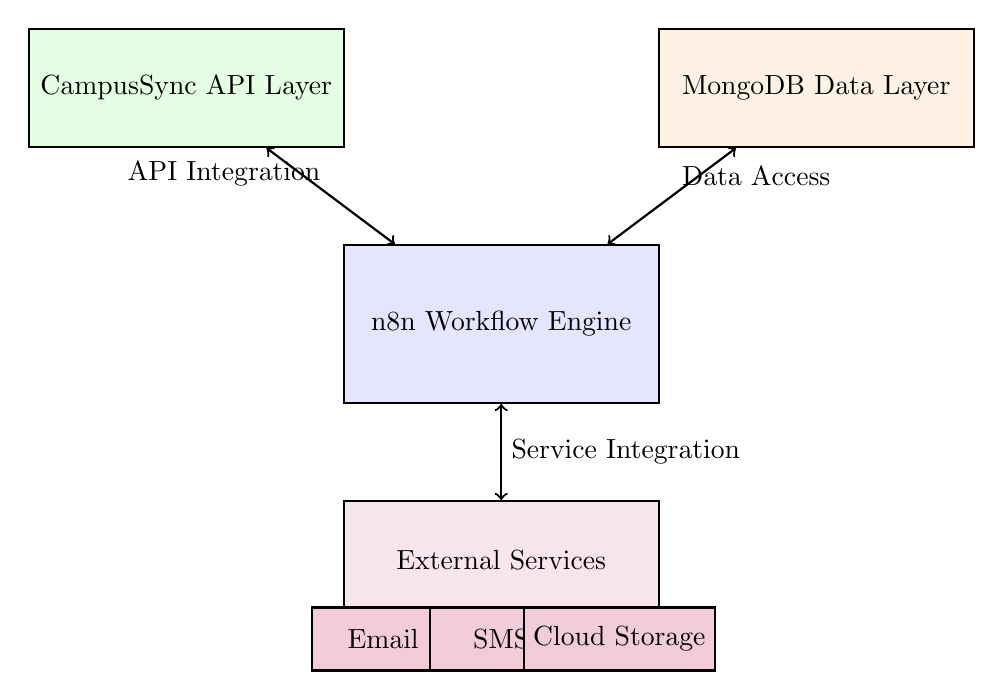
\begin{tikzpicture}[thick]
        % n8n Workflow Engine
        \node[draw, rectangle, minimum width=4cm, minimum height=2cm, fill=blue!10] (n8n) at (0,0) {n8n Workflow Engine};
        
        % CampusSync API
        \node[draw, rectangle, minimum width=4cm, minimum height=1.5cm, fill=green!10] (api) at (-4,3) {CampusSync API Layer};
        
        % Database
        \node[draw, rectangle, minimum width=4cm, minimum height=1.5cm, fill=orange!10] (database) at (4,3) {MongoDB Data Layer};
        
        % External Services
        \node[draw, rectangle, minimum width=4cm, minimum height=1.5cm, fill=purple!10] (external) at (0,-3) {External Services};
        \node[draw, rectangle, minimum width=1.8cm, minimum height=0.8cm, fill=purple!20] (email) at (-1.5,-4) {Email};
        \node[draw, rectangle, minimum width=1.8cm, minimum height=0.8cm, fill=purple!20] (sms) at (0,-4) {SMS};
        \node[draw, rectangle, minimum width=1.8cm, minimum height=0.8cm, fill=purple!20] (cloud) at (1.5,-4) {Cloud Storage};
        
        % Arrows
        \draw[<->] (api) -- (n8n) node[midway, above left] {API Integration};
        \draw[<->] (database) -- (n8n) node[midway, above right] {Data Access};
        \draw[<->] (n8n) -- (external) node[midway, right] {Service Integration};
    \end{tikzpicture}
    \caption{n8n Integration Architecture}
    \label{fig:n8n-integration}
\end{figure}

\section{Enterprise Communication Integration}

\subsection{Email Integration}

The platform will integrate with enterprise email services to provide robust communication capabilities:

\subsubsection{Service Providers}

\begin{itemize}
    \item \textbf{Primary}: SendGrid (High deliverability, advanced analytics)
    \item \textbf{Secondary}: Amazon SES (Cost-effective, scalable)
    \item \textbf{Tertiary}: Mailgun (Redundancy, global delivery)
\end{itemize}

\subsubsection{Advanced Email Features}

\begin{itemize}
    \item \textbf{Dynamic Template Engine}: Role-specific content personalization
    \item \textbf{Behavioral Triggering}: Event-based communication workflows
    \item \textbf{Delivery Scheduling}: Time-zone aware message optimization
    \item \textbf{Comprehensive Analytics}: Real-time engagement metrics and A/B testing
    \item \textbf{Compliance Management}: GDPR/FERPA compliant communication protocols
\end{itemize}

\subsection{SMS Integration}

Global SMS integration will provide instant communication capabilities:

\subsubsection{Service Provider Ecosystem}

\begin{itemize}
    \item \textbf{Global Coverage}: Twilio (99.9\% uptime, extensive network)
    \item \textbf{Regional Optimization}: Vonage (Cost-effective local routing)
    \item \textbf{Emergency Redundancy}: Plivo (Backup communication channel)
\end{itemize}

\subsubsection{Enterprise SMS Capabilities}

\begin{itemize}
    \item \textbf{Priority Queuing}: Mission-critical message prioritization
    \item \textbf{Multi-Factor Authentication}: Secure access verification protocols
    \item \textbf{Emergency Broadcasting}: Instant mass-notification system
    \item \textbf{Delivery Scheduling}: Time-zone optimized message delivery
    \item \textbf{Cost Optimization}: Intelligent routing for economical delivery
\end{itemize}

\section{External Service Integration}

Campus-Sync will integrate with various external services to extend its capabilities and provide a more comprehensive educational environment.

\subsection{Learning Management Ecosystem}

\begin{itemize}
    \item \textbf{Google Classroom}: Seamless content and assignment synchronization
    \item \textbf{Microsoft Teams}: Native integration with Office 365 environments
    \item \textbf{Canvas/Moodle}: Bidirectional data exchange and interoperability
\end{itemize}

\subsection{Productivity Platform Integration}

\begin{itemize}
    \item \textbf{Google Workspace}: Calendar, Drive, and Docs synchronization
    \item \textbf{Microsoft 365}: Teams, Outlook, and SharePoint connectivity
    \item \textbf{Slack/Discord}: Community engagement and collaboration channels
\end{itemize}

\subsection{Financial Services Integration}

\begin{itemize}
    \item \textbf{Stripe/PayPal}: Multi-channel payment processing
    \item \textbf{Regional Payment Gateways}: Local payment method support
    \item \textbf{Accounting Systems}: QuickBooks, Xero integration for financial reporting
\end{itemize}

\subsection{Cloud Storage Federation}

\begin{itemize}
    \item \textbf{Google Drive}: Document management and sharing
    \item \textbf{Dropbox}: Enterprise file synchronization
    \item \textbf{OneDrive}: Microsoft ecosystem integration
    \item \textbf{Box}: Enterprise-grade content management
\end{itemize}

\section{Advanced Automation Scenarios}

\subsection{Intelligence Workflows}

\begin{itemize}
    \item \textbf{Administrative Risk Assessment}: Machine learning-based institutional efficiency prediction
    \item \textbf{Teacher Adaptive Learning Paths}: Dynamic curriculum adjustment algorithms
    \item \textbf{Student Resource Allocation}: Demand forecasting and optimization
    \item \textbf{Cross-Panel Personalized Recommendations}: AI-driven content and activity suggestions
\end{itemize}

\subsection{Context-Aware Communication}

\begin{itemize}
    \item \textbf{Location-Based Notifications}: Geo-fencing for campus services
    \item \textbf{Behavioral Pattern Recognition}: Usage-based engagement optimization
    \item \textbf{Collaborative Workflows}: Cross-panel project coordination
    \item \textbf{Feedback-Driven Improvement}: Continuous system optimization
\end{itemize}

\section{Enterprise Security and Compliance}

Future implementations will enhance security and compliance capabilities to meet enterprise standards.

\subsection{Data Protection Protocols}

\begin{itemize}
    \item \textbf{End-to-End Encryption}: AES-256 communication security
    \item \textbf{Role-Based Access Control}: Granular permission management by panel
    \item \textbf{Comprehensive Audit Trails}: Complete action logging and tracking
    \item \textbf{Regulatory Compliance}: GDPR, FERPA, HIPAA alignment
\end{itemize}

\subsection{Authentication Security}

\begin{itemize}
    \item \textbf{OAuth 2.0 Integration}: Secure third-party service authentication
    \item \textbf{API Key Management}: Rotating credential security protocols
    \item \textbf{Rate Limiting}: Abuse prevention and system protection
    \item \textbf{Real-Time Monitoring}: Anomaly detection and threat response
\end{itemize}

\section{Implementation Roadmap}

The future development of Campus-Sync follows a phased approach to ensure smooth integration and minimal disruption to existing operations.

\subsection{Phase 1: Foundation (Months 1-2)}

\begin{itemize}
    \item n8n infrastructure provisioning and configuration
    \item Core email and SMS service integration
    \item Basic notification workflow deployment
    \item Monitoring and analytics framework establishment
\end{itemize}

\subsection{Phase 2: Administrative Enhancement (Months 3-4)}

\begin{itemize}
    \item Comprehensive administrative workflow automation
    \item User management and course planning automation
    \item Report generation and analytics implementation
    \item Delivery optimization and performance tuning
\end{itemize}

\subsection{Phase 3: Teacher Integration (Months 5-6)}

\begin{itemize}
    \item Teacher workflow automation deployment
    \item Assignment and grade processing automation
    \item Class communication and analytics implementation
    \item Enhanced security protocol deployment
\end{itemize}

\subsection{Phase 4: Student Optimization (Months 7-8)}

\begin{itemize}
    \item Student engagement automation systems
    \item Academic progress tracking and alerts
    \item Wellness and productivity integration
    \item User experience optimization initiatives
\end{itemize}

\subsection{Phase 5: Cross-Panel Integration (Months 9-12)}

\begin{itemize}
    \item Cross-panel workflow orchestration
    \item AI-powered automation workflows
    \item Productivity platform integration
    \item Comprehensive monitoring dashboard launch
\end{itemize}

\section{Investment Analysis}

\subsection{Operational Expenditure}

\begin{itemize}
    \item \textbf{n8n Hosting}: \$50-200/month (scalable infrastructure)
    \item \textbf{Communication Services}: \$100-300/month (email/SMS volume-based)
    \item \textbf{API Integration}: \$50-150/month (third-party service fees)
    \item \textbf{Monitoring Tools}: \$50-100/month (analytics and observability)
\end{itemize}

\subsection{Resource Investment}

\begin{itemize}
    \item \textbf{Infrastructure}: Dedicated automation server resources
    \item \textbf{Development}: Specialized workflow engineering personnel
    \item \textbf{Operations}: System monitoring and maintenance staff
    \item \textbf{Support}: User assistance for automated features
\end{itemize}

\section{Key Performance Indicators}

\subsection{Quantitative Metrics}

\begin{itemize}
    \item \textbf{Operational Efficiency}: Hours saved through process automation
    \item \textbf{User Engagement}: Platform usage increase and retention rates
    \item \textbf{Communication Effectiveness}: Improved delivery and response metrics
    \item \textbf{Error Reduction}: Decreased manual intervention requirements
\end{itemize}

\subsection{Qualitative Assessments}

\begin{itemize}
    \item \textbf{User Satisfaction}: Stakeholder feedback and satisfaction scores
    \item \textbf{Administrative Productivity}: Staff efficiency and workflow improvements
    \item \textbf{Academic Outcomes}: Measurable impact on student performance
    \item \textbf{System Reliability}: Uptime, performance, and scalability metrics
\end{itemize}

\section{Emerging Technology Integration}

\subsection{Future Expansion Opportunities}

\begin{itemize}
    \item \textbf{Machine Learning}: Advanced predictive analytics and automation
    \item \textbf{Internet of Things}: Smart campus device and sensor integration
    \item \textbf{Blockchain}: Immutable academic credential verification
    \item \textbf{Immersive Technologies}: AR/VR-enhanced learning experiences
\end{itemize}

\subsection{Market Development}

\begin{itemize}
    \item \textbf{Corporate Education}: Enterprise training platform adaptation
    \item \textbf{Primary/Secondary Education}: K-12 optimized feature sets
    \item \textbf{Higher Education}: Research-focused advanced capabilities
    \item \textbf{Global Markets}: Localization and international compliance
\end{itemize}

\section{Conclusion}

The future development roadmap for Campus-Sync positions the platform as a next-generation educational solution. By leveraging cutting-edge automation technologies, enterprise-grade communication systems, and strategic external service integrations, Campus-Sync will continue to evolve into an intelligent, efficient, and engaging learning environment.

The integration of n8n workflow automation, comprehensive communication systems, and advanced security measures will establish Campus-Sync as a leader in educational technology innovation. This strategic enhancement roadmap ensures that the platform remains at the forefront of educational technology while meeting the evolving needs of students, teachers, and administrators in the digital age.